\documentclass{article}
\usepackage[utf8]{inputenc}
\usepackage[margin=1.2in]{geometry}
\usepackage{amsmath, amssymb, amsthm, graphicx, float}
\usepackage{subfig, subfloat}
\allowdisplaybreaks

\title{MengProject}
\author{Arjun Jauhari }
\date{March 2016}

\begin{document}

\maketitle

\section{Data}
\begin{figure}[h]
\centering
\includegraphics[width=15cm]{stackexchange.png}
\caption{Sample Graph}
\label{fig1:overview}
\end{figure}
Data is structured into following files
\begin{itemize}
    \item Badges.xml
    \item \textbf{Comments.xml}
    \item PostHistory.xml
    \item PostLinks.xml
    \item \textbf{Posts.xml}
    \item Tags.xml
    \item \textbf{Users.xml}
    \item Votes.xml
\end{itemize}

A typical row in Posts.xml file looks like \\

$<row \textbf{Id}="1" \textbf{PostTypeId}="1" \textbf{CreationDate}="2015-02-03T16:40:26.487" \textbf{Score}="22" \textbf{ViewCount}="307" \textbf{Body}="Sample Question" \textbf{OwnerUserId}="2" \textbf{LastEditorUserId}="2" \textbf{LastEditDate}="2015-02-03T17:51:07.583" \textbf{LastActivityDate}="2015-02-03T21:05:27.990" \textbf{Title}="Sample Title" \textbf{Tags}="line-numbers" \textbf{AnswerCount}="2" \textbf{CommentCount}="0" \textbf{FavoriteCount}="3" />$


\section{Extracting Attributes}
Wrote shell scripts to extract out the attributes from the above mentioned data files. Attributes used for the project were:
\subsection{From Posts.xml file}
Id\\
PostTypeId\\
OwnerUserId\\
ParentId(onlyforans)\\
Score\\
AcceptedAnswerId\\
CreationDate\\
AnswerCount\\
\subsection{From Users.xml file}
Id\\
DisplayName\\
Reputation\\
UpVotes\\
DownVotes\\
\subsection{From Votes.xml file}
Id\\
PostId\\
VoteTypeId\\
CreationDate\\

\section{Generating Gephi graphs}
\begin{figure}[h]
\centering
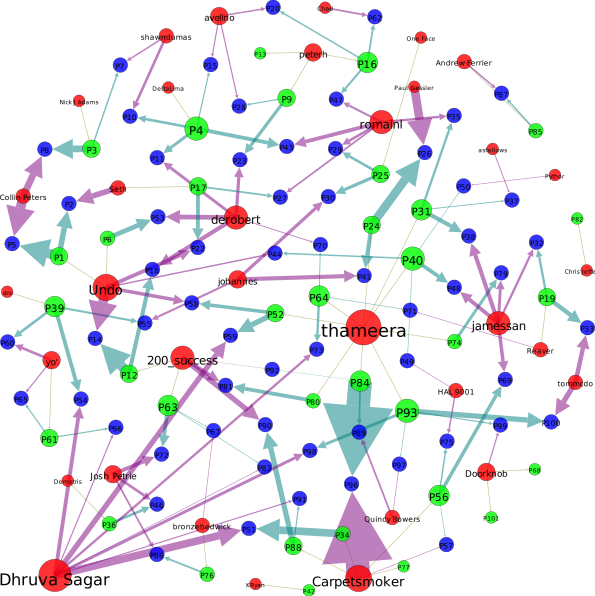
\includegraphics[width=9cm]{proposalimg.png}
\caption{Sample Graph}
\label{fig1:overview}
\end{figure}
To visualise this model I generated graphs using Gephi, figure 1 above
shows one graph on a very small subset of data. Legend for the graph-
\begin{itemize}
    \item Red Nodes: User
    \item Green Nodes: Questions
    \item Blue Nodes: Answers
    \item Green Edge: User2Question(u2q)
    \item Blue Edge: User2Answer(u2b)
    \item Grey Edge: Question2Answer(q2a)
\end{itemize}
The edges connect each user to their post.
Post can be a question(green edge) or an answer(blue edge).
Also, each question is connected to its answers through grey edge.\\
\\
Important details about the graph -
\begin{itemize}
    \item Node size represents, how active is that particular user. For example, user
        with name 'thameera' is the one of the most active user followed by user
        'Dhruv Sagar'.
    \item The thickness of these q2a edges tells the quality of an answer relative to 
all the other answers for same parent question. For example, user 'Carpet Smoker' has
        give one of the best answer.
\end{itemize}

\section{Modelling as System of Linear Equations}
\subsection{Subscripts}
\begin{itemize}
    \item $i$ is subscript for question.
    \item $j$ is subscript for answer.
    \item $k$ is subscript for user.
\end{itemize}
\subsection{Notations}
\begin{enumerate}
    \item $u_k$: Quality measure of the $k$th user.
    \item $q_i$: Quality measure of the $i$th question.
    \item $va_{ij}$: Normalized votes corresponding to $j$th answer of $i$th question. \\
        Calculated as: $va_{ij} = \frac{|sa_{ij}|}{\sum_{j} |sa_{ij}|}$ \\
        where $sa_{ij}$ is the actual votes(score) read from data dump.
    \item $a_{ijk}$: Quality measure of $a_{ij}$th answer given by the $k$th user.
    \item $f_{acc}^{ij}$: Boolean flag telling if this answer was Accepted, read from data dump.
    \item $r_k$: Reputation of the $k$th user, read from data dump.
    \item $N_{a}^{i}$: Number of answer to $i$th question, read from data dump.
    \item $vq_{i}$: Number of votes to $i$th question, read from data dump.
\end{enumerate}

\subsection{Equations}
Below equations model the relation/dependence between
the above defined parameters. \\
Bold values are known features.
All the features were scaled between 0 \& 1 \\
\begin{enumerate}
    \item $a_{ijk} = f_a(u_k, \mathbf{va_{ij}}, \mathbf{f_{acc}^{ij}})$ \\
        $a_{ijk} = 1/3*u_k + 1/3*\mathbf{va_{ij}} + 1/3*\mathbf{f_{acc}^{ij}}$
    \item $u_k = f_u(\{a_{ijk}\}_{ij}, \{q_i\}_k, \mathbf{r_k})$ , where $\{a_{ijk}\}_{ij}$
        is set of all answers by user k\\
        $u_k = 1/3*mean\{a_{ijk}\}_{ij} + 1/3*mean\{q_i\}_k + 1/3*\mathbf{r_k}$
    \item $q_i = f_q(u_k, \mathbf{N_{a}^{i}}, \mathbf{vq_i}, \mathbf{\sum_{j} |sa_{ij}|})$, where $\sum_{j} |sa_{ij}|$
        is sum of votes for all the answers of $i$th question \\
        $q_i = 1/4*u_k + 1/4*\mathbf{N_{a}^{i}}+ 1/4* \mathbf{vq_i} + 1/4*\mathbf{\sum_{j} |sa_{ij}|}$
\end{enumerate}

\subsection{Solving this model}
All the above 3 set of equations are combined together to form a system of linear
equations. \\
$Ax = B$, where $A$ is the coefficient matrix and $B$ is the vector of all the 
known quantities. $x$ is the vector of all the unknowns namely : $a_{ijk}, u_k, q_i$

\subsection{Results from this model}
Structure of typical $A$ matrix looks like: (white = positive, black=negative, grey = zero)
\begin{figure}[h]
\centering
\includegraphics[width=12cm]{result_LS/hintonAmat.png}
\caption{Sample Graph}
\label{fig1:overview}
\end{figure}
\\
Precision at K plot, where K is number of Users being considered
\begin{figure}[h]
\centering
\includegraphics[width=12cm]{result_LS/PatK.png}
\caption{Sample Graph}
\label{fig1:overview}
\end{figure}
\\
Histogram of User quality and question quality
\begin{figure}[H]
\centering
\includegraphics[width=12cm]{result_LS/UQualHist.png}
\caption{Sample Graph}
\label{fig1:overview}
\end{figure}
\begin{figure}[H]
\centering
\includegraphics[width=12cm]{result_LS/QQualHist.png}
\caption{Sample Graph}
\label{fig1:overview}
\end{figure}

\newpage
\section{Probabilistic Graphical Model based approach}
\subsection{Preprocess data}
Pre-processed data files to Structure them into useful data structures which can
be used in model simulation.\\
One of the main data structure was a dictionary mapping each question to its 
click history. For example, \\
\{Q1 : list of click History\}. \\
Further click History was structured as list of list \\
$[[vote1, [list of answers present]], [vote2, [...]], ...] $ \\
Note: Each click can either be an UpVote or DownVote.\\

\section{Model Simulation}
\subsection{Graphical Model}
Below is the graphical model used. Red node color corresponds to observed variable.
\begin{figure}[H]
\centering
\includegraphics[width=12cm]{gm.png}
\caption{Sample Graph}
\label{fig1:overview}
\end{figure}

\subsection{Equations}
Goal is to find the probability $P(\theta, \phi | clicks)$ \\
And by Bayes rule, \\
\begin{equation*}
\begin{split}
    &P(\theta, \phi | clicks) \propto P(clicks | \theta, \phi) * P(\theta,\phi)\\
    &P(\theta, \phi | clicks) \propto P(clicks | \theta, \phi) * P(\theta | \phi)
    * P(\theta)\\
    \\
\end{split}
\end{equation*}\\

Now, we defined the conditional probability as \\
\begin{equation*}
\begin{split}
    &P(click = k | \theta_1, ..., \theta_n) = \frac{exp(\theta_k)}{exp(\theta_1) + ... + exp(\theta_n)} \\
\end{split}
\end{equation*}\\
and \\
\begin{equation*}
\begin{split}
    &P(\theta_i | \phi_j) \sim \mathcal{N}(\phi_j, \sigma^2) \\
    &P(\theta_i | \phi_j) = \frac{1}{\sqrt{2\pi\sigma^2}} exp(\frac{-|\theta_i - \phi_j|^2}{2\sigma^2}) \\
\end{split}
\end{equation*}\\
and \\
\begin{equation*}
\begin{split}
    &P(\phi_j) \sim \mathcal{N}(0, \sigma^2) \\
\end{split}
\end{equation*}\\

\subsection{Objective Function}
The objective function is the product of the 3 terms defined above for every 
$user(\phi), answer(\theta)$ and $click(k)$. \\ 

The goal is to minimize this function and we explored several gradient descent based
optimization methods. \\
\textbf{L-BFGS} : Limited-memory BFGS (L-BFGS or LM-BFGS) is an optimization 
algorithm in the family of quasi-Newton methods that approximates the 
Broyden–Fletcher–Goldfarb–Shanno (BFGS) algorithm using a limited amount
of computer memory. It is a popular algorithm for parameter estimation in 
machine learning. \\
\textbf{AdaGrad} : AdaGrad (for adaptive gradient algorithm) is a modified 
stochastic gradient descent with per-parameter learning rate, first 
published in 2011. Informally, this increases the learning 
rate for more sparse parameters and decreases the learning rate for less 
sparse ones. This strategy often improves convergence performance over 
standard stochastic gradient descent in settings where data is sparse and 
sparse parameters are more informative. \\

\section{Moving to BIG DATA}
Till now all the experiments were based on data set from smaller stack exchange
websites like "http://vi.stackexchange.com/" and "http://datascience.stackexchange.com/".
In these websites the Number of Users were around 13,000 and number of Posts were
around 7,000 and the data set size was $\sim$ 15MB.\\

Once the model was tested on smaller websites, we moved to our final target i.e.
"stackoverflow.com", which has \\
\begin{itemize}
    \item Number of Users = 5277830 ($\sim$ 5 million), file size 1.5GB
    \item Number of Posts(Question + Answers) = 29499662 ($\sim$ 30 million), file size 45GB
    \item Number of Votes = 98928934 ($\sim$ 99 million), file size 9GB
\end{itemize}
Total dataset size of $\sim$ 55GB

To process this huge dataset, I broke each file into multiple smaller files and 
processed one at a time. As the whole big file was not fitting into the memory of 
system.\\
\section{Visualization and Results}
\subsection{Simulation Results}
Below results validates the correctness of the implementation of model.\\
\begin{figure}[h]
\centering
\includegraphics[width=12cm]{results_ver2/KTau-User.png}
\caption{Sample Graph}
\label{fig1:overview}
\end{figure}

\subsection{Real data TimeLine View}
\begin{figure}[H]
\centering
\includegraphics[width=12cm]{results_ver2/downVote_TL.png}
\caption{Sample Graph}
\label{fig1:overview}
\end{figure}
\begin{figure}[H]
\centering
\includegraphics[width=12cm]{results_ver2/downVote_SOL.png}
\caption{Sample Graph}
\label{fig1:overview}
\end{figure}
\begin{figure}[H]
\centering
\includegraphics[width=12cm]{results_ver2/longVote_TL.png}
\caption{Sample Graph}
\label{fig1:overview}
\end{figure}
\begin{figure}[H]
\centering
\includegraphics[width=12cm]{results_ver2/longVote_SOL.png}
\caption{Sample Graph}
\label{fig1:overview}
\end{figure}
\begin{figure}[H]
\centering
\includegraphics[width=12cm]{results_ver2/timeWeightTL.png}
\caption{Sample Graph}
\label{fig1:overview}
\end{figure}
\begin{figure}[H]
\centering
\includegraphics[width=12cm]{results_ver2/timeWeightSol.png}
\caption{Sample Graph}
\label{fig1:overview}
\end{figure}

\subsection{Statistics from BIG DATA}
\begin{figure}[H]
\centering
\includegraphics[width=12cm]{results_ver2/so_user_cum_hist.png}
\caption{Sample Graph}
\label{fig1:overview}
\end{figure}
\begin{figure}[H]
\centering
\includegraphics[width=12cm]{results_ver2/so_user_postcnt_hist.png}
\caption{Sample Graph}
\label{fig1:overview}
\end{figure}
\begin{figure}[H]
\centering
\includegraphics[width=12cm]{results_ver2/so_user_quescnt_hist.png}
\caption{Sample Graph}
\label{fig1:overview}
\end{figure}
\begin{figure}[H]
\centering
\includegraphics[width=12cm]{results_ver2/so_user_anscnt_hist.png}
\caption{Sample Graph}
\label{fig1:overview}
\end{figure}

\end{document}


